\documentclass{beamer}
\usepackage[utf8]{inputenc}

\usetheme{Madrid}
\usecolortheme{default}
\usepackage{amsmath,amssymb,amsfonts,amsthm}
\usepackage{txfonts}
\usepackage{tkz-euclide}
\usepackage{listings}
\usepackage{adjustbox}
\usepackage{array}
\usepackage{tabularx}
\usepackage{gvv}
\usepackage{lmodern}
\usepackage{circuitikz}
\usepackage{tikz}
\usepackage{graphicx}

\setbeamertemplate{page number in head/foot}[totalframenumber]

\usepackage{tcolorbox}
\tcbuselibrary{minted,breakable,xparse,skins}



\definecolor{bg}{gray}{0.95}
\DeclareTCBListing{mintedbox}{O{}m!O{}}{%
  breakable=true,
  listing engine=minted,
  listing only,
  minted language=#2,
  minted style=default,
  minted options={%
    linenos,
    gobble=0,
    breaklines=true,
    breakafter=,,
    fontsize=\small,
    numbersep=8pt,
    #1},
  boxsep=0pt,
  left skip=0pt,
  right skip=0pt,
  left=25pt,
  right=0pt,
  top=3pt,
  bottom=3pt,
  arc=5pt,
  leftrule=0pt,
  rightrule=0pt,
  bottomrule=2pt,

  colback=bg,
  colframe=orange!70,
  enhanced,
  overlay={%
    \begin{tcbclipinterior}
    \fill[orange!20!white] (frame.south west) rectangle ([xshift=20pt]frame.north west);
    \end{tcbclipinterior}},
  #3,
}
\lstset{
    language=C,
    basicstyle=\ttfamily\small,
    keywordstyle=\color{blue},
    stringstyle=\color{orange},
    commentstyle=\color{green!60!black},
    numbers=left,
    numberstyle=\tiny\color{gray},
    breaklines=true,
    showstringspaces=false,
}
%------------------------------------------------------------
%This block of code defines the information to appear in the
%Title page
\title %optional
{2.10.42}
\date{September  2025}
%\subtitle{A short story}

\author % (optional)
{BEERAM MADHURI - EE25BTECH11012}

\begin{document}


\frame{\titlepage}
\begin{frame}{Question}
If $\mathbf{a}, \mathbf{b}$ and $\mathbf{c}$ are unit coplanar vectors, then the scalar triple product
\[\begin{bmatrix}2\mathbf{a} - \mathbf{b} & 2\mathbf{b} - \mathbf{c} & 2\mathbf{c} - \mathbf{a}\end{bmatrix} =\]
\end{frame}
  
\begin{frame}{solution}
\frametitle{finding scalar triple product of \[\begin{bmatrix}2\mathbf{a} - \mathbf{b} & 2\mathbf{b} - \mathbf{c} & 2\mathbf{c} - \mathbf{a}\end{bmatrix} \] }
\begin{align}
\vec{B} = (2\vec{a} - \vec{b} \quad 2\vec{b} - \vec{c} \quad 2\vec{c} - \vec{a}) = (\vec{a} \quad \vec{b} \quad \vec{c})\begin{pmatrix}2 & 0 & -1 \\-1 & 2 & 0 \\0 & -1 & 2\end{pmatrix}
\end{align}

Since $\vec{a}$, $\vec{b}$, $\vec{c}$ are coplanar,
\begin{align}
\begin{vmatrix}\vec{a} & \vec{b} & \vec{c}\end{vmatrix} = 0
\end{align}
\begin{align}
    \begin{vmatrix}2\vec{a} - \vec{b} & 2\vec{b} - \vec{c} & 2\vec{c} - \vec{a}\end{vmatrix} = \begin{vmatrix}\vec{a} & \vec{b} & \vec{c}\end{vmatrix} \begin{vmatrix}2 & 0 & -1 \\-1 & 2 & 0 \\0 & -1 & 2\end{vmatrix} =0
\end{align}

Hence, the value of $\begin{bmatrix} 2\vec{a} - \vec{b} & 2\vec{b} - \vec{c} & 2\vec{c} - \vec{a}\end{bmatrix}$ = 0.
\end{frame}
\begin{frame}
\[\text {Proof of } \begin{bmatrix} \vec{a} & \vec{b} & \vec{c} \end{bmatrix} \text{ is singular:}\]
Given $\vec{a}$,$\vec{b}$,$\vec{c}$ are coplanar\\
plane equation of the plane through  $\vec{a}$,$\vec{b}$,$\vec{c}$ be 
\begin{align}
\vec{n}^\top \vec{r} = 0
\end{align}
where $\vec{n}$ is normal to plane
\begin{align}
\vec{n}^\top \Vec{a} &= 0 \\ 
\vec{n}^\top \vec{b} &= 0 \\
\vec{n}^\top \vec{c} &= 0
\end{align}
\end{frame}
\begin{frame}
let $M = \begin{bmatrix} \vec{a} & \vec{b} & \vec{c} \end{bmatrix}$
\begin{align}
\vec{n}^\top M = 0^\top
\end{align}
For a homogeneous linear system
\begin{align}
\vec{n}^\top M = 0^\top, \quad \mathbf{n} \neq 0
\end{align}
$M$ must be singular.

\[\therefore \begin{bmatrix} \vec{a} & \vec{b} & \vec{c}  \end{bmatrix} \text{ is singular}\]
Hence proved
\end{frame}


\begin{frame}[fragile]
    \frametitle{Python Code}
    \begin{lstlisting}
import matplotlib.pyplot as plt
import numpy as np

# Create a 3D plot
fig = plt.figure(figsize=(10, 8))
ax = fig.add_subplot(111, projection='3d')

\end{lstlisting}
\end{frame}

\begin{frame}[fragile]
    \frametitle{Python Code}
    \begin{lstlisting}
# --- 1. Define three unit coplanar vectors (a, b, c) ---
# For simplicity, we'll place them on the x-y plane (z=0).
# These are just example vectors that satisfy the conditions.
a = np.array([1, 0, 0])
b = np.array([np.cos(np.pi/3), np.sin(np.pi/3), 0])  # 60 degrees from a
c = np.array([np.cos(2*np.pi/3), np.sin(2*np.pi/3), 0]) # 120 degrees from a
v1 = 2 * a - b
v2 = 2 * b - c
v3 = 2 * c - a

    \end{lstlisting}
\end{frame}
\begin{frame}[fragile]
    \frametitle{Python Code}

    \begin{lstlisting}
# --- 3. Plot the vectors ---
origin = np.array([0, 0, 0])
ax.quiver(*origin, *a, color='r', label='a', arrow_length_ratio=0.1)
ax.quiver(*origin, *b, color='g', label='b', arrow_length_ratio=0.1)
ax.quiver(*origin, *c, color='b', label='c', arrow_length_ratio=0.1)
ax.quiver(*origin, *v1, color='orange', label='v1 = 2a - b', arrow_length_ratio=0.1, linestyle='--')
ax.quiver(*origin, *v2, color='purple', label='v2 = 2b - c', arrow_length_ratio=0.1, linestyle='--')
ax.quiver(*origin, *v3, color='cyan', label='v3 = 2c - a', arrow_length_ratio=0.1, linestyle='--')

    \end{lstlisting}
\end{frame}

\begin{frame}[fragile]
    \frametitle{Python Code}

    \begin{lstlisting}
# --- 4. Add labels for each vector ---
ax.text(*(a*1.1), 'a', color='r', fontsize=12)
ax.text(*(b*1.1), 'b', color='g', fontsize=12)
ax.text(*(c*1.1), 'c', color='b', fontsize=12)
ax.text(*(v1*1.05), 'v1', color='orange', fontsize=12)
ax.text(*(v2*1.05), 'v2', color='purple', fontsize=12)
ax.text(*(v3*1.05), 'v3', color='cyan', fontsize=12)
\end{lstlisting}
\end{frame}

 
\begin{frame}[fragile]
    \frametitle{Python Code}
    \begin{lstlisting}
# --- 5. Visualize the plane ---
# Create a grid for the plane at z=0
xx, yy = np.meshgrid(np.linspace(-3, 3, 2), np.linspace(-3, 3, 2))
zz = np.zeros_like(xx)
ax.plot_surface(xx, yy, zz, alpha=0.1, color='gray')

\end{lstlisting}
\end{frame}

\begin{frame}[fragile]
    \frametitle{Python Code}
    \begin{lstlisting}
# --- 6. Set plot aesthetics ---
ax.set_xlim([-3, 3])
ax.set_ylim([-3, 3])
ax.set_zlim([-3, 3])
ax.set_xlabel('X axis')
ax.set_ylabel('Y axis')
ax.set_zlabel('Z axis')
ax.set_title('Visualization of Coplanar Vectors')
ax.legend()
ax.grid(True)
# Set a viewing angle for better perspective
ax.view_init(elev=25, azim=30)
plt.show()
\end{lstlisting}
\end{frame}

\begin{frame}[fragile]
\frametitle{C Code}
\begin{lstlisting}
#include <stdio.h>

typedef struct {
    double x, y, z;
} Vector;
Vector createVector(double x, double y, double z) {
    Vector v = {x, y, z};
    return v;
}
Vector subtract(Vector u, Vector v) {
    return createVector(u.x - v.x, u.y - v.y, u.z - v.z);
}
Vector scale(Vector u, double k) {
    return createVector(k*u.x, k*u.y, k*u.z);
}
\end{lstlisting}

\end{frame}
\begin{frame}[fragile]
\frametitle{C Code}
\begin{lstlisting}
   Vector cross(Vector u, Vector v) {
    return createVector(
        u.y*v.z - u.z*v.y,
        u.z*v.x - u.x*v.z,
        u.x*v.y - u.y*v.x
    );
}
double dot(Vector u, Vector v) {
    return u.x*v.x + u.y*v.y + u.z*v.z;
}
double triple(Vector u, Vector v, Vector w) {
    return dot(u, cross(v, w));
}
\end{lstlisting}
\end{frame}
\begin{frame}[fragile]
\frametitle{C Code}
\begin{lstlisting}
Vector twominus(Vector a, Vector b) {
    return subtract(scale(a, 2), b); }
double computeX(Vector a, Vector b, Vector c) {
    Vector v1 = twominus(a, b);
    Vector v2 = twominus(b, c);
    Vector v3 = twominus(c, a);
    return triple(v1, v2, v3);}
__attribute__((visibility("default"))) 
double computeX_py(double ax, double ay, double az,
                   double bx, double by, double bz,
                   double cx, double cy, double cz) {
    Vector a = createVector(ax, ay, az);
    Vector b = createVector(bx, by, bz);
    Vector c = createVector(cx, cy, cz);
    return computeX(a, b, c);}
\end{lstlisting}

\end{frame}


\begin{frame}[fragile]
\frametitle{Python and C Code}

\begin{lstlisting}
import ctypes

lib = ctypes.CDLL("./libscalartp.so")

lib.computeX_py.argtypes = [ctypes.c_double, ctypes.c_double, ctypes.c_double,
                            ctypes.c_double, ctypes.c_double, ctypes.c_double,
                            ctypes.c_double, ctypes.c_double, ctypes.c_double]
lib.computeX_py.restype = ctypes.c_double

a = (1.0, 0.0, 0.0)
b = (0.0, 1.0, 0.0)
c = (0.6,0.8,0)

X = lib.computeX_py(*a, *b, *c)
print("X =", X)
\end{lstlisting}
\end{frame}

\begin{frame}
\begin{figure}[H]
    \centering
    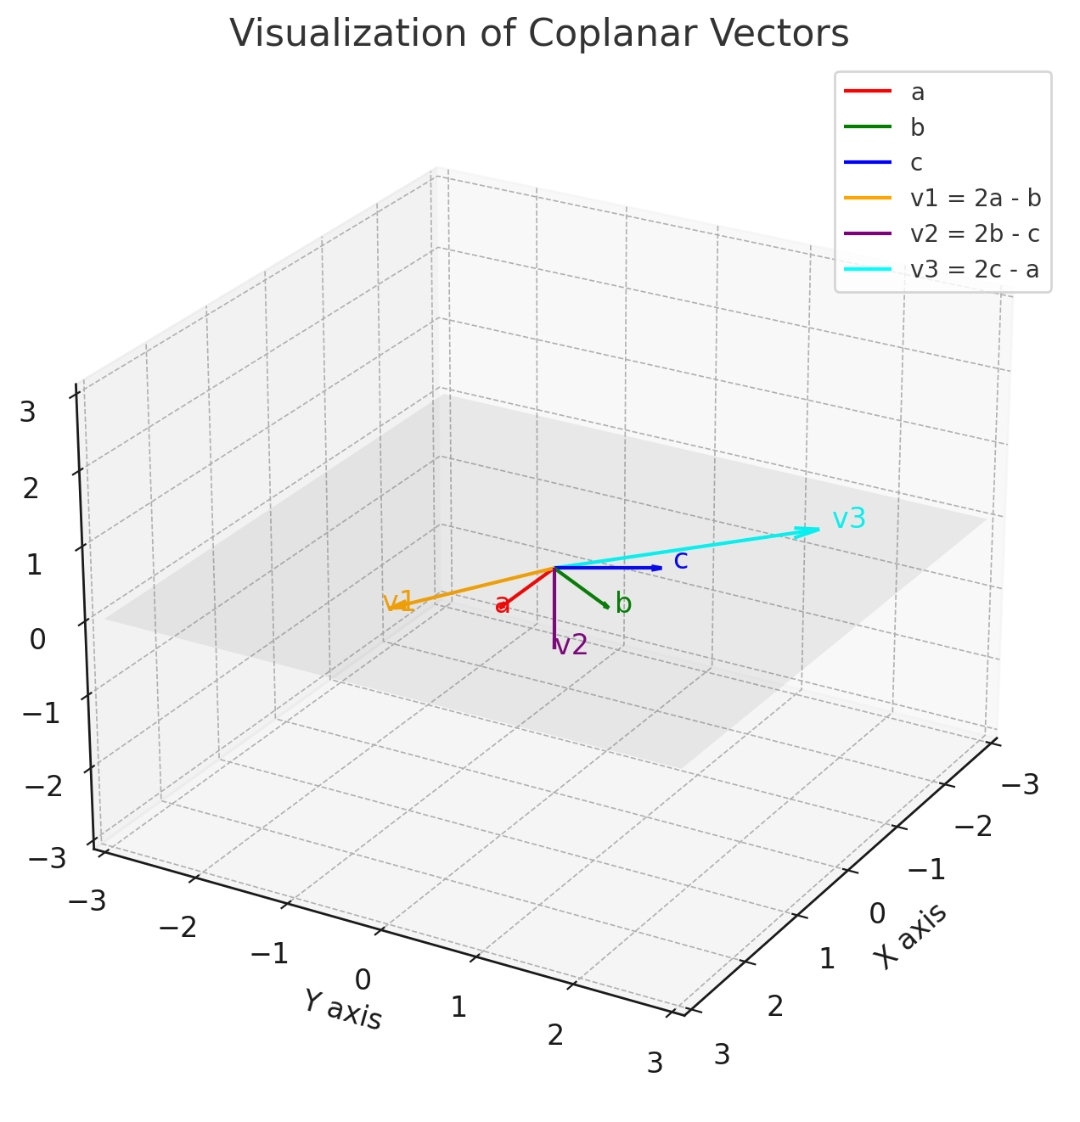
\includegraphics[width=0.7\columnwidth]{graph-1.png}
    \caption{Plot}
    \label{fig:placeholder}
\end{figure}
\end{frame}

\end{document}